\lab{Algorithms}{Speeding up Python Functions: Vectorization}{Vectorization One}

\objective{Demonstrates the importance of vectorization.}

This lab introduces two applied topics (Information Entropy and Chebyshev Polynomials) to explore how we can make functions faster through vectorization. There are two primary motivations behind vectorizing code.  First, vectorized code is often much clearer and more concise than non-vectorized code.  The second, much larger motivation is performance.  Vectorized code is often order of magnitudes faster than non-vectorized code.

The concept behind vectorizing code is to move away from operating on one element at a time and toward operating on entire collections of elements at once.  This section will focus specifically on reducing the number of for loops in our program.  Let us look at two examples of functions that would be really useful if we could vectorize them to make them execute faster.

\section*{Information Entropy}

Information entropy is loosely defined as the amount of information that is encoded in each bit of a signal. It is directly related to amount of compression that a signal can undergo without loss.

For example, suppose that our signal is an infinite string ``AAAAAAA..." Since the signal never changes, each additional bit after the first adds no new information. Thus the entropy in this case is zero.

On the other hand, we assign a truly random uniform binary source an entropy of one (such a source may be related to radioactive decay). The reason for this is that we have absolutely no clue what the next symbol we read will be.

We can empirically calculate the entropy of a given signal by the following:
\begin{equation*}
H = -\sum_k{p_k \log_2(p_k)}
\end{equation*}
where $p_k$ is the probability of the $k^{th}$ symbol. Note that this fits the two conventions we set above since
\begin{equation*}
-(1\cdot\log_2(1) + 0\cdot\log_2(0)) = 0
\end{equation*}
\begin{equation*}
-(\frac{1}{2}\log_2\frac{1}{2} + \frac{1}{2}\log_2\frac{1}{2}) = 1
\end{equation*}

\begin{problem}
Write a function that finds the entropy of an array (you will need to flatten multidimensional arrays to a single dimension). You will also need to empirically calculate the probability of a given symbol (start by letting your symbols be integers). To find the probability of a symbol, you need to find the number of times it occurs in the sequence and divide it by the length of the sequence (watch out for integer division).
\end{problem}

We can test the entropy function that you just wrote against bit sources to see how ``random" they are. For example, we can read an image into Python and view it using the following code:
\begin{lstlisting}
>>> from scipy import misc
>>> img = misc.imread('cameraman.tif'); img
\end{lstlisting}

\begin{figure}[h!]
\begin{center}
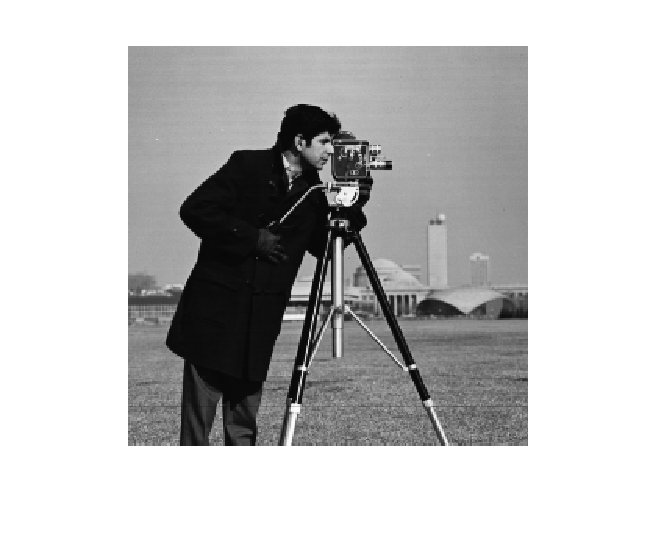
\includegraphics{cameramanClean.pdf}
\end{center}
\caption{The MIT Camera Man, a classic image used in image processing}
\label{fig:cameramanclean}
\end{figure}

You should see the image shown in Figure \ref{fig:cameramanclean}. Now pass this image to the entropy function to calculate the entropy of the image data. We get a value of $7.009$. If this image were uniformly random, the entropy would be $8$, since each pixel is an $8$ bit number, and a uniform distribution of integers between $1$ and $128 = 2^8$ will have an entropy of $8$ (you can verify this fairly easily using the equation we defined above). This implies that the image has potential for compression.

\begin{problem}
Now rewrite your function without using loops. This is an example of using vectorization to speed up algorithms. Use the cameraman image to test how much faster this function is than the original.
\end{problem}

\section*{Chebyshev Polynomials}

One special class of polynomials is the class of Chebyshev Polynomials. They are useful in a variety of applications including:
\begin{itemize}
\item Evaluating integrals using Gaussian quadrature
\item Solving partial differential equations
\item Speeding up iterative matrix methods (finding eigenvalues and solving large systems)
\item Minimizing interpolation error
\end{itemize}

We will explain many of the these applications in subsequent chapters. The purpose of this example is for you to investigate ways to speed up a process on your own.

The $n^{th}$ Chebyshev Polynomial can be described equivalently by the following formulae\footnotemark :
\begin{equation*}
T_n(x) = \cos(n \cos^{-1}(x))
\end{equation*}
\begin{equation*}
T_n(x) = 2xT_{n-1}(x) - T_{n-2}(x), T_0(x) = 1, T_1(x) = x
\end{equation*}

\footnotetext{Technically the first formula only works on the interval $[-1,1]$. There are more general formulae, piecewise defined using $\cosh$ outside of $[-1,1]$, but for this exercise we'll stick to the above definition.}

\begin{problem}
Write a function that accepts a vector $x_0$ of values in $[-1,1]$ and a degree $n$.  The function should return an array evaluating each entry of $x_0$ at every Chebyshev polynomial of degree $n$ or less. The $n^{th}$ column of the output should contain the $n-1$ Chebyshev Polynomial evaluated at $x_0$.

You will be writing four slightly different versions of this function.
\begin{enumerate}
\item Use only for-loops and Python's \li{math} library (you will need two for-loops).
\item Same as previous, but replacing one for loop with a list comprehension.
\item Use \li{numpy.vectorize} to vectorize Python's \li{math} functions.  Keep the list comprehension from previous part.
\item Use SciPy's optimized $\cos$ and $\arccos$ functions.
\end{enumerate}

Make this function as fast as possible. You should investigate both mathematical definitions, and how the number of for-loops affects the speed.
\end{problem}
